% Drawing 74/07-6 -- folder 74, batch 07, archive page 131 (PDF page 132).
% Transcription: un point $a$ et un triangle.
% Kind: triangle and a point. Method 2 (schematic redraw from the facsimile). Status: ok.
% Notes: A triangle in bold strokes and a point to its lower right; the letter under it is read as a (as in the transcription) with doubt.
% Coordinates: 1 unit = 1 mm = 1/100 of the crop width (bbox in page fractions: [0.18, 0.57, 0.32, 0.64]).
% Redrawn by Claude (claude-opus-5-5), issue #73, 2026-11-07; not checked by a human; not compiled (no TeX in the session).
% Rights: reproduces part of the work -- behind RENDER_TRANSCRIPTS, never published by itself.
\documentclass[tikz,border=3pt]{standalone}
\usepackage{amsmath,amssymb}
\usetikzlibrary{patterns,arrows.meta}
\tikzset{pencil/.style={black!45}, struck/.style={black!35}, mark/.style={circle,draw,inner sep=1.3pt}, pt/.style={circle,fill,inner sep=0.9pt}, opt/.style={circle,draw,fill=white,inner sep=1.1pt}}
\begin{document}
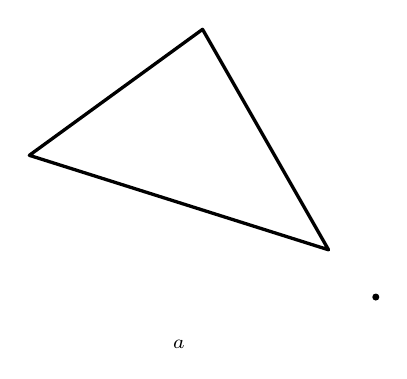
\begin{tikzpicture}[x=1mm,y=1mm,line cap=round,line join=round,font=\scriptsize]
\draw[very thick] (42,-38) -- (64,-22) -- (80,-50) -- cycle;
\node[pt] at (86,-56) {};
\node[inner sep=1pt] at (61,-62) {\scriptsize $a$};
\end{tikzpicture}
\end{document}
